\question Theorem 8 states that: If a graph \(G\) is a subdivision of a graph \(H\), then \(H\) is a minor of \(G\). Give an example that its converse is false.

\begin{solution}
  Consider the following graphs \(H\) and \(G\). Note that both graphs are
  simple graphs.
  
  \begin{center}
    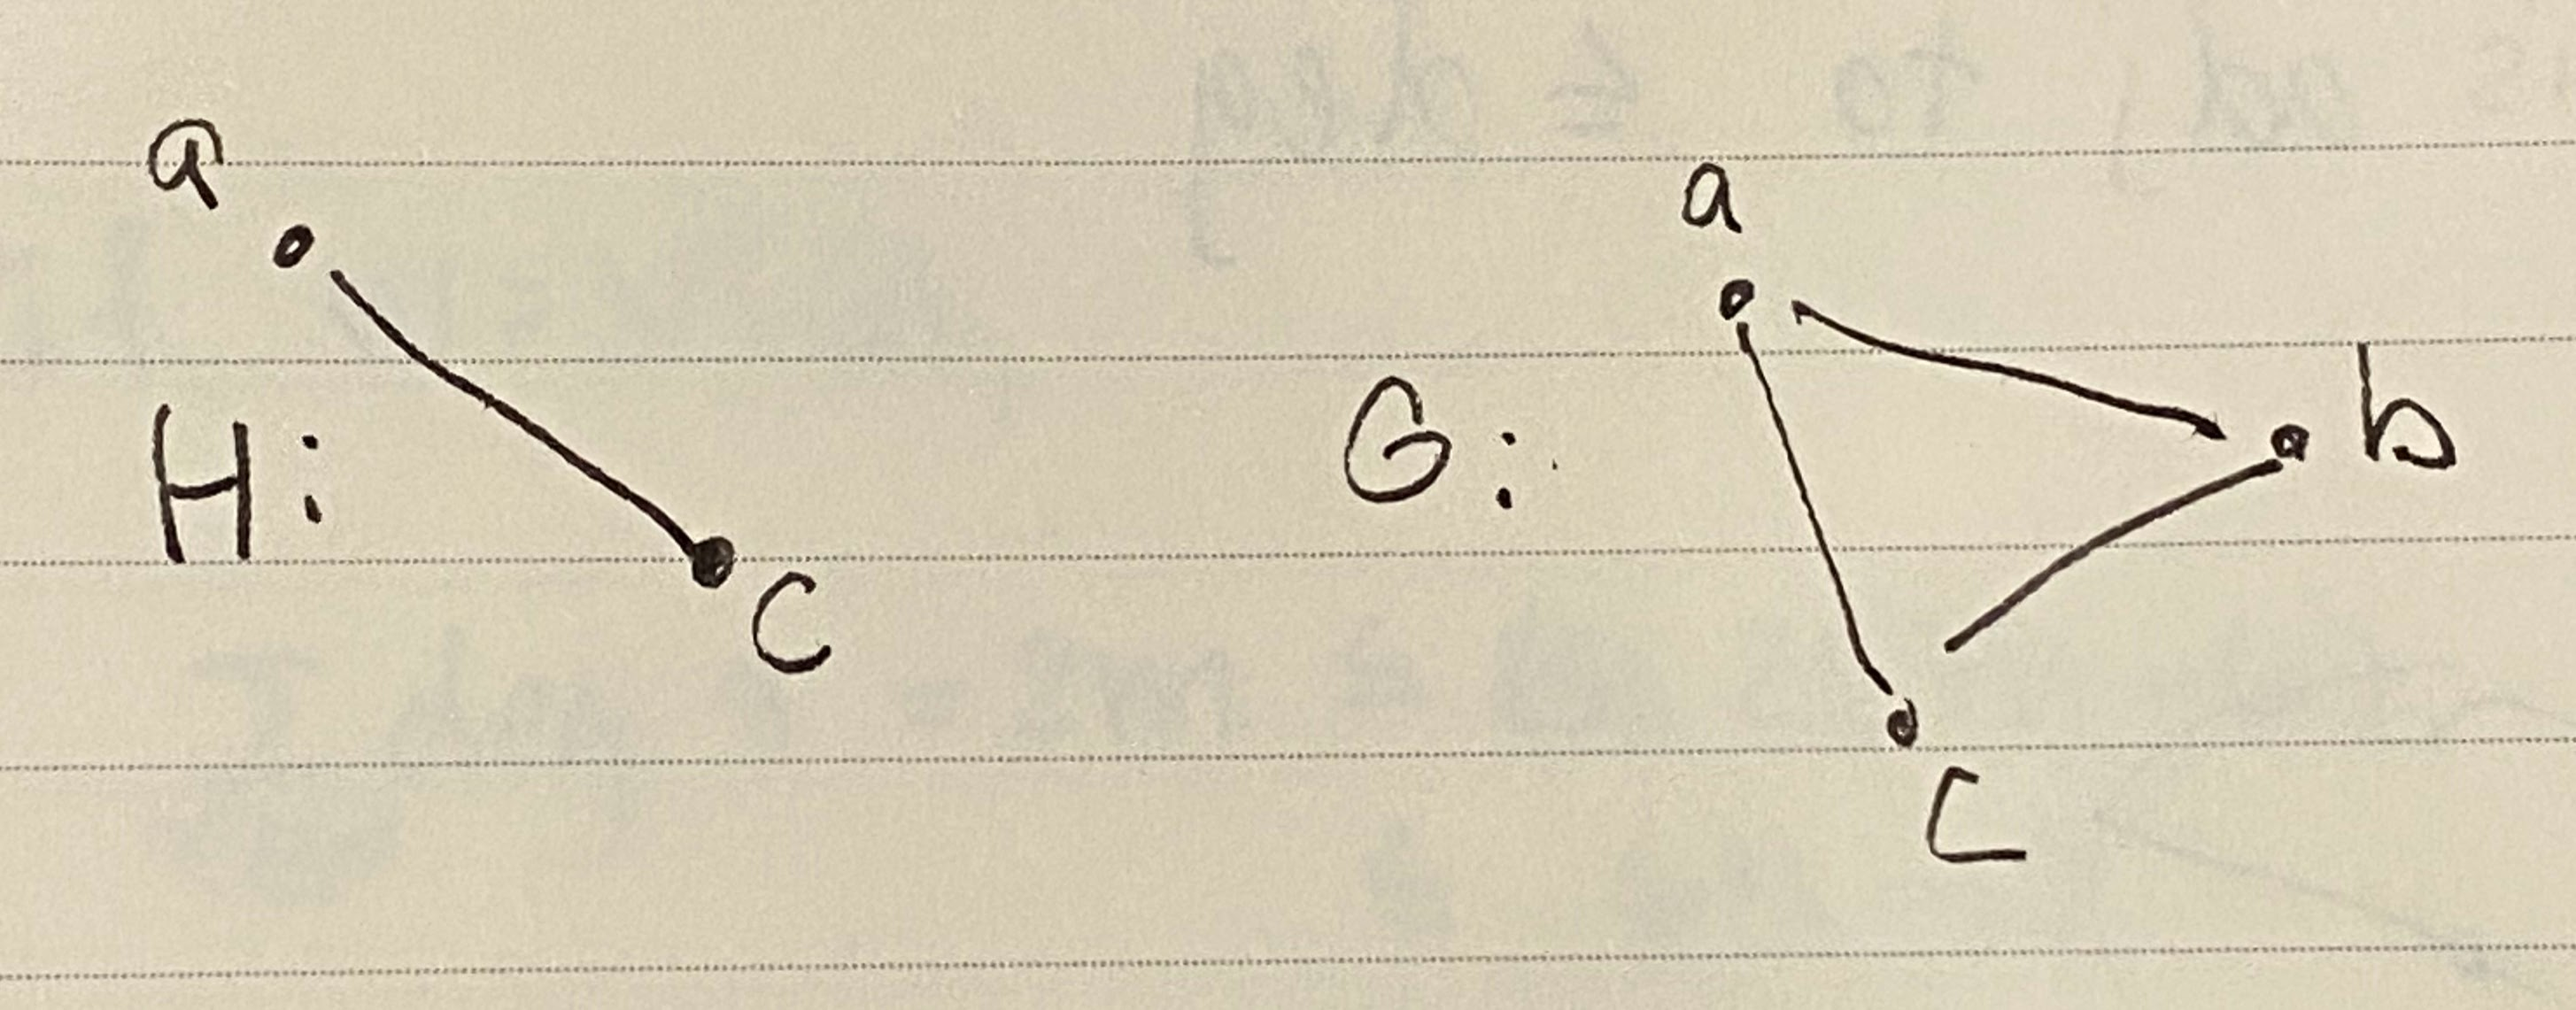
\includegraphics[width=0.69\textwidth]{figures/IMG_7890}
  \end{center}

  We can see that \(H\) is a minor of \(G\) by contracting either the edge
  \(ab\) or \(cb\) in \(G\). However, any subdivision of \(H\), say \(H'\), will
  only have extra vertices on the \(ac\) edge but no \(ac\) edge can exist in
  \(H'\) unlike in \(G\).
\end{solution}
